\documentclass[1p]{elsarticle_modified}
%\bibliographystyle{elsarticle-num}

%\usepackage[colorlinks]{hyperref}
%\usepackage{abbrmath_seonhwa} %\Abb, \Ascr, \Acal ,\Abf, \Afrak
\usepackage{amsfonts}
\usepackage{amssymb}
\usepackage{amsmath}
\usepackage{amsthm}
\usepackage{scalefnt}
\usepackage{amsbsy}
\usepackage{kotex}
\usepackage{caption}
\usepackage{subfig}
\usepackage{color}
\usepackage{graphicx}
\usepackage{xcolor} %% white, black, red, green, blue, cyan, magenta, yellow
\usepackage{float}
\usepackage{setspace}
\usepackage{hyperref}

\usepackage{tikz}
\usetikzlibrary{arrows}

\usepackage{multirow}
\usepackage{array} % fixed length table
\usepackage{hhline}

%%%%%%%%%%%%%%%%%%%%%
\makeatletter
\renewcommand*\env@matrix[1][\arraystretch]{%
	\edef\arraystretch{#1}%
	\hskip -\arraycolsep
	\let\@ifnextchar\new@ifnextchar
	\array{*\c@MaxMatrixCols c}}
\makeatother %https://tex.stackexchange.com/questions/14071/how-can-i-increase-the-line-spacing-in-a-matrix
%%%%%%%%%%%%%%%

\usepackage[normalem]{ulem}

\newcommand{\msout}[1]{\ifmmode\text{\sout{\ensuremath{#1}}}\else\sout{#1}\fi}
%SOURCE: \msout is \stkout macro in https://tex.stackexchange.com/questions/20609/strikeout-in-math-mode

\newcommand{\cancel}[1]{
	\ifmmode
	{\color{red}\msout{#1}}
	\else
	{\color{red}\sout{#1}}
	\fi
}

\newcommand{\add}[1]{
	{\color{blue}\uwave{#1}}
}

\newcommand{\replace}[2]{
	\ifmmode
	{\color{red}\msout{#1}}{\color{blue}\uwave{#2}}
	\else
	{\color{red}\sout{#1}}{\color{blue}\uwave{#2}}
	\fi
}

\newcommand{\Sol}{\mathcal{S}} %segment
\newcommand{\D}{D} %diagram
\newcommand{\A}{\mathcal{A}} %arc


%%%%%%%%%%%%%%%%%%%%%%%%%%%%%5 test

\def\sl{\operatorname{\textup{SL}}(2,\Cbb)}
\def\psl{\operatorname{\textup{PSL}}(2,\Cbb)}
\def\quan{\mkern 1mu \triangleright \mkern 1mu}

\theoremstyle{definition}
\newtheorem{thm}{Theorem}[section]
\newtheorem{prop}[thm]{Proposition}
\newtheorem{lem}[thm]{Lemma}
\newtheorem{ques}[thm]{Question}
\newtheorem{cor}[thm]{Corollary}
\newtheorem{defn}[thm]{Definition}
\newtheorem{exam}[thm]{Example}
\newtheorem{rmk}[thm]{Remark}
\newtheorem{alg}[thm]{Algorithm}

\newcommand{\I}{\sqrt{-1}}
\begin{document}

%\begin{frontmatter}
%
%\title{Boundary parabolic representations of knots up to 8 crossings}
%
%%% Group authors per affiliation:
%\author{Yunhi Cho} 
%\address{Department of Mathematics, University of Seoul, Seoul, Korea}
%\ead{yhcho@uos.ac.kr}
%
%
%\author{Seonhwa Kim} %\fnref{s_kim}}
%\address{Center for Geometry and Physics, Institute for Basic Science, Pohang, 37673, Korea}
%\ead{ryeona17@ibs.re.kr}
%
%\author{Hyuk Kim}
%\address{Department of Mathematical Sciences, Seoul National University, Seoul 08826, Korea}
%\ead{hyukkim@snu.ac.kr}
%
%\author{Seokbeom Yoon}
%\address{Department of Mathematical Sciences, Seoul National University, Seoul, 08826,  Korea}
%\ead{sbyoon15@snu.ac.kr}
%
%\begin{abstract}
%We find all boundary parabolic representation of knots up to 8 crossings.
%
%\end{abstract}
%\begin{keyword}
%    \MSC[2010] 57M25 
%\end{keyword}
%
%\end{frontmatter}

%\linenumbers
%\tableofcontents
%
\newcommand\colored[1]{\textcolor{white}{\rule[-0.35ex]{0.8em}{1.4ex}}\kern-0.8em\color{red} #1}%
%\newcommand\colored[1]{\textcolor{white}{ #1}\kern-2.17ex	\textcolor{white}{ #1}\kern-1.81ex	\textcolor{white}{ #1}\kern-2.15ex\color{red}#1	}

{\Large $\underline{12a_{0753}~(K12a_{0753})}$}

\setlength{\tabcolsep}{10pt}
\renewcommand{\arraystretch}{1.6}
\vspace{1cm}\begin{tabular}{m{100pt}>{\centering\arraybackslash}m{274pt}}
\multirow{5}{120pt}{
	\centering
	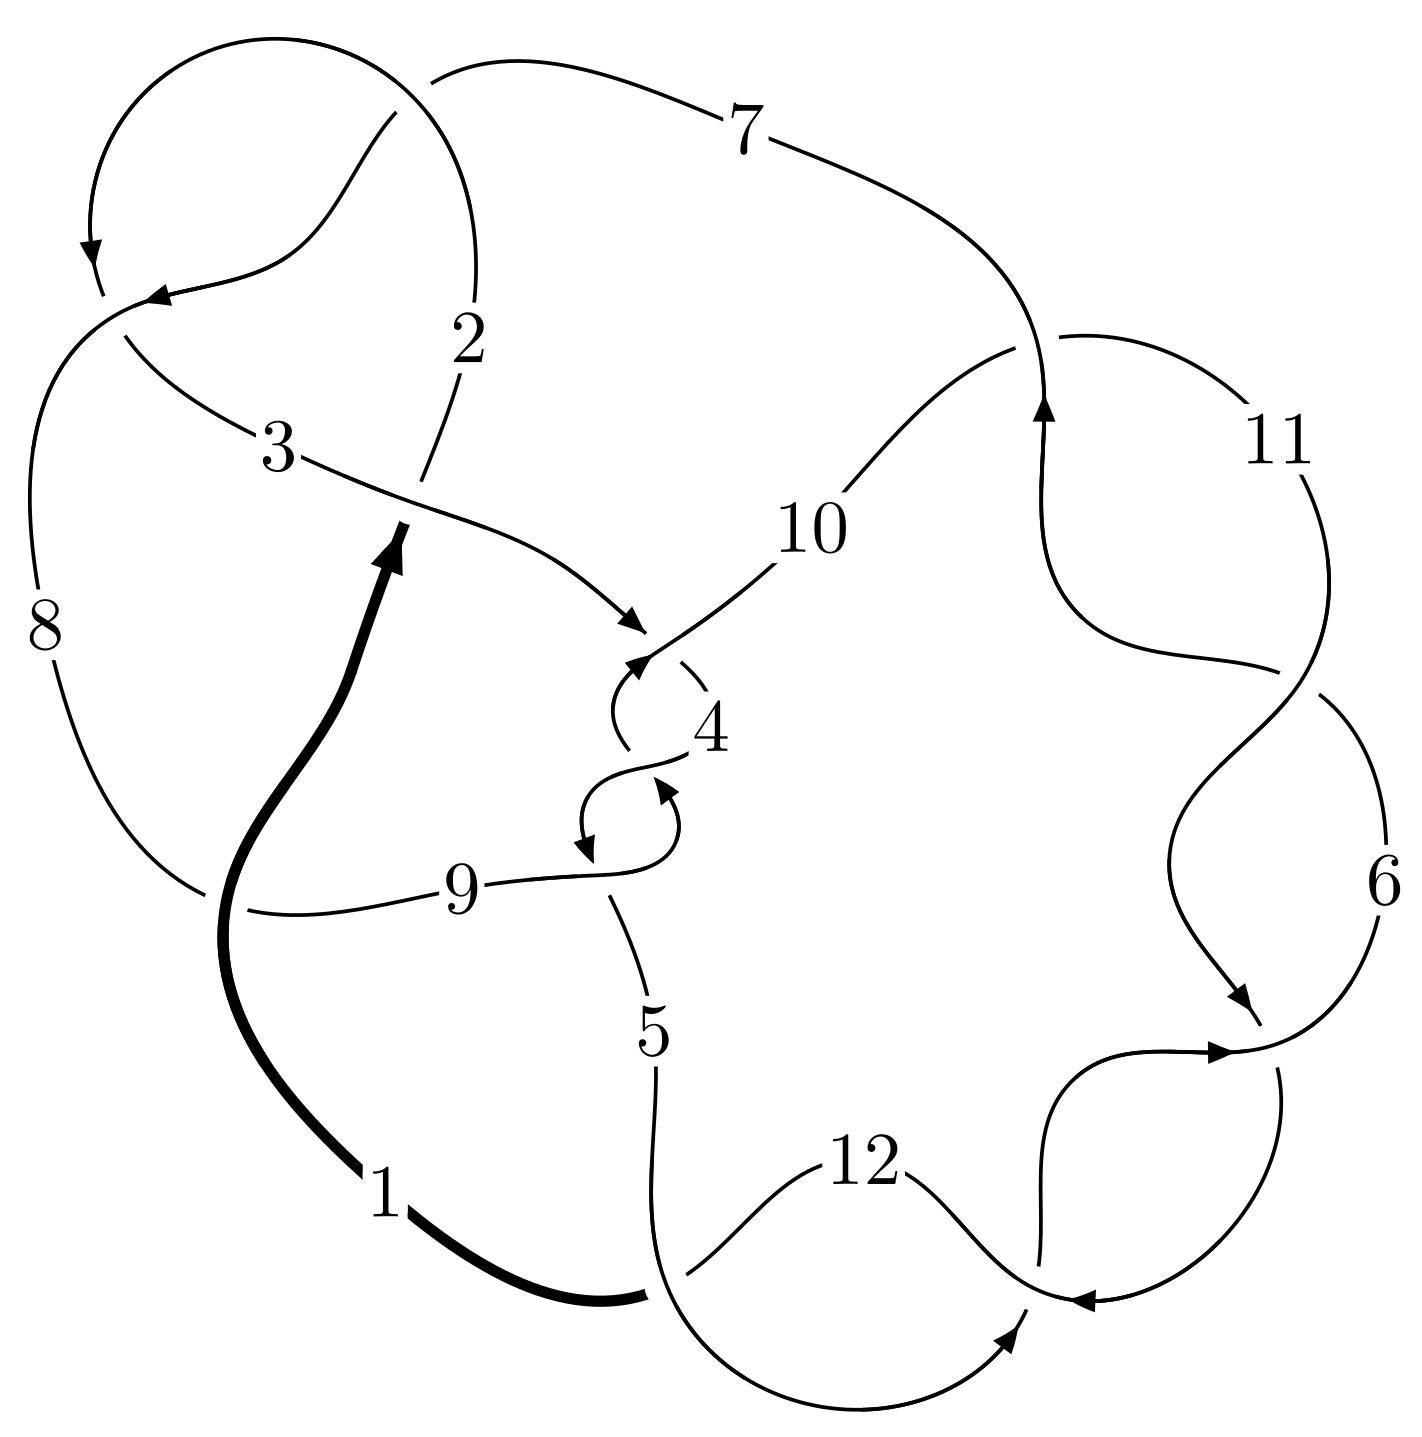
\includegraphics[width=112pt]{../../../GIT/diagram.site/Diagrams/png/1554_12a_0753.png}\\
\ \ \ A knot diagram\footnotemark}&
\allowdisplaybreaks
\textbf{Linearized knot diagam} \\
\cline{2-2}
 &
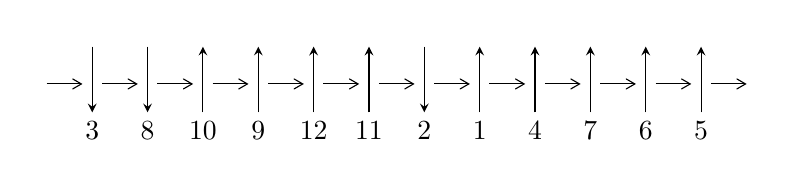
\begin{tikzpicture}[x=20pt, y=17pt]
	% nodes
	\node (C0) at (0, 0) {};
	\node (C1) at (1, 0) {};
	\node (C1U) at (1, +1) {};
	\node (C1D) at (1, -1) {3};

	\node (C2) at (2, 0) {};
	\node (C2U) at (2, +1) {};
	\node (C2D) at (2, -1) {8};

	\node (C3) at (3, 0) {};
	\node (C3U) at (3, +1) {};
	\node (C3D) at (3, -1) {10};

	\node (C4) at (4, 0) {};
	\node (C4U) at (4, +1) {};
	\node (C4D) at (4, -1) {9};

	\node (C5) at (5, 0) {};
	\node (C5U) at (5, +1) {};
	\node (C5D) at (5, -1) {12};

	\node (C6) at (6, 0) {};
	\node (C6U) at (6, +1) {};
	\node (C6D) at (6, -1) {11};

	\node (C7) at (7, 0) {};
	\node (C7U) at (7, +1) {};
	\node (C7D) at (7, -1) {2};

	\node (C8) at (8, 0) {};
	\node (C8U) at (8, +1) {};
	\node (C8D) at (8, -1) {1};

	\node (C9) at (9, 0) {};
	\node (C9U) at (9, +1) {};
	\node (C9D) at (9, -1) {4};

	\node (C10) at (10, 0) {};
	\node (C10U) at (10, +1) {};
	\node (C10D) at (10, -1) {7};

	\node (C11) at (11, 0) {};
	\node (C11U) at (11, +1) {};
	\node (C11D) at (11, -1) {6};

	\node (C12) at (12, 0) {};
	\node (C12U) at (12, +1) {};
	\node (C12D) at (12, -1) {5};
	\node (C13) at (13, 0) {};

	% arrows
	\draw[->,>={angle 60}]
	(C0) edge (C1) (C1) edge (C2) (C2) edge (C3) (C3) edge (C4) (C4) edge (C5) (C5) edge (C6) (C6) edge (C7) (C7) edge (C8) (C8) edge (C9) (C9) edge (C10) (C10) edge (C11) (C11) edge (C12) (C12) edge (C13) ;	\draw[->,>=stealth]
	(C1U) edge (C1D) (C2U) edge (C2D) (C3D) edge (C3U) (C4D) edge (C4U) (C5D) edge (C5U) (C6D) edge (C6U) (C7U) edge (C7D) (C8D) edge (C8U) (C9D) edge (C9U) (C10D) edge (C10U) (C11D) edge (C11U) (C12D) edge (C12U) ;
	\end{tikzpicture} \\
\hhline{~~} \\& 
\textbf{Solving Sequence} \\ \cline{2-2} 
 &
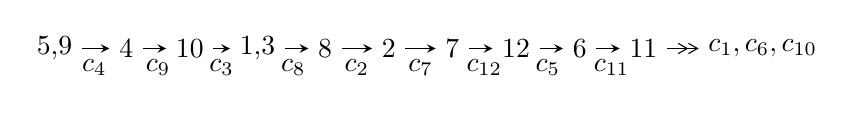
\begin{tikzpicture}[x=23pt, y=7pt]
	% node
	\node (A0) at (-1/8, 0) {5,9};
	\node (A1) at (1, 0) {4};
	\node (A2) at (2, 0) {10};
	\node (A3) at (49/16, 0) {1,3};
	\node (A4) at (33/8, 0) {8};
	\node (A5) at (41/8, 0) {2};
	\node (A6) at (49/8, 0) {7};
	\node (A7) at (57/8, 0) {12};
	\node (A8) at (65/8, 0) {6};
	\node (A9) at (73/8, 0) {11};
	\node (C1) at (1/2, -1) {$c_{4}$};
	\node (C2) at (3/2, -1) {$c_{9}$};
	\node (C3) at (5/2, -1) {$c_{3}$};
	\node (C4) at (29/8, -1) {$c_{8}$};
	\node (C5) at (37/8, -1) {$c_{2}$};
	\node (C6) at (45/8, -1) {$c_{7}$};
	\node (C7) at (53/8, -1) {$c_{12}$};
	\node (C8) at (61/8, -1) {$c_{5}$};
	\node (C9) at (69/8, -1) {$c_{11}$};
	\node (A10) at (11, 0) {$c_{1},c_{6},c_{10}$};

	% edge
	\draw[->,>=stealth]	
	(A0) edge (A1) (A1) edge (A2) (A2) edge (A3) (A3) edge (A4) (A4) edge (A5) (A5) edge (A6) (A6) edge (A7) (A7) edge (A8) (A8) edge (A9) ;
	\draw[->>,>={angle 60}]	
	(A9) edge (A10);
\end{tikzpicture} \\ 

\end{tabular} \\

\footnotetext{
The image of knot diagram is generated by the software ``\textbf{Draw programme}" developed by Andrew Bartholomew(\url{http://www.layer8.co.uk/maths/draw/index.htm\#Running-draw}), where we modified some parts for our purpose(\url{https://github.com/CATsTAILs/LinksPainter}).
}\phantom \\ \newline 
\centering \textbf{Ideals for irreducible components\footnotemark of $X_{\text{par}}$} 
 
\begin{align*}
I^u_{1}&=\langle 
3.47678\times10^{21} u^{49}-1.33799\times10^{21} u^{48}+\cdots+1.34820\times10^{22} b-3.88891\times10^{22},\\
\phantom{I^u_{1}}&\phantom{= \langle  }2.21158\times10^{21} u^{49}-1.62283\times10^{21} u^{48}+\cdots+1.34820\times10^{22} a-4.79098\times10^{22},\;u^{50}- u^{49}+\cdots-4 u+4\rangle \\
I^u_{2}&=\langle 
b^2- b u+1,\;a^2+a+1,\;u^2+1\rangle \\
\\
\end{align*}
\raggedright * 2 irreducible components of $\dim_{\mathbb{C}}=0$, with total 58 representations.\\
\footnotetext{All coefficients of polynomials are rational numbers. But the coefficients are sometimes approximated in decimal forms when there is not enough margin.}
\newpage
\renewcommand{\arraystretch}{1}
\centering \section*{I. $I^u_{1}= \langle 3.48\times10^{21} u^{49}-1.34\times10^{21} u^{48}+\cdots+1.35\times10^{22} b-3.89\times10^{22},\;2.21\times10^{21} u^{49}-1.62\times10^{21} u^{48}+\cdots+1.35\times10^{22} a-4.79\times10^{22},\;u^{50}- u^{49}+\cdots-4 u+4 \rangle$}
\flushleft \textbf{(i) Arc colorings}\\
\begin{tabular}{m{7pt} m{180pt} m{7pt} m{180pt} }
\flushright $a_{5}=$&$\begin{pmatrix}1\\0\end{pmatrix}$ \\
\flushright $a_{9}=$&$\begin{pmatrix}0\\u\end{pmatrix}$ \\
\flushright $a_{4}=$&$\begin{pmatrix}1\\u^2\end{pmatrix}$ \\
\flushright $a_{10}=$&$\begin{pmatrix}u\\u^3+u\end{pmatrix}$ \\
\flushright $a_{1}=$&$\begin{pmatrix}-0.164040 u^{49}+0.120370 u^{48}+\cdots+8.84293 u+3.55361\\-0.257882 u^{49}+0.0992428 u^{48}+\cdots+2.87776 u+2.88452\end{pmatrix}$ \\
\flushright $a_{3}=$&$\begin{pmatrix}u^2+1\\u^4+2 u^2\end{pmatrix}$ \\
\flushright $a_{8}=$&$\begin{pmatrix}0.570562 u^{49}-0.676764 u^{48}+\cdots-8.50993 u-2.63929\\0.00372260 u^{49}+0.222580 u^{48}+\cdots-6.74010 u-1.68097\end{pmatrix}$ \\
\flushright $a_{2}=$&$\begin{pmatrix}0.137529 u^{49}-0.0400013 u^{48}+\cdots+4.53679 u+1.15498\\-0.233430 u^{49}+0.0703666 u^{48}+\cdots+1.46685 u+2.29315\end{pmatrix}$ \\
\flushright $a_{7}=$&$\begin{pmatrix}0.836099 u^{49}-0.448168 u^{48}+\cdots-24.1572 u-6.13765\\-0.144284 u^{49}+0.0267194 u^{48}+\cdots-0.748206 u-1.92710\end{pmatrix}$ \\
\flushright $a_{12}=$&$\begin{pmatrix}0.0938429 u^{49}+0.0211270 u^{48}+\cdots+5.96518 u+0.669092\\-0.257882 u^{49}+0.0992428 u^{48}+\cdots+2.87776 u+2.88452\end{pmatrix}$ \\
\flushright $a_{6}=$&$\begin{pmatrix}0.122630 u^{49}-0.215276 u^{48}+\cdots-0.518300 u-8.94249\\0.297613 u^{49}-0.201245 u^{48}+\cdots-3.06461 u+0.521412\end{pmatrix}$ \\
\flushright $a_{11}=$&$\begin{pmatrix}-0.0377076 u^{49}-0.204943 u^{48}+\cdots-5.37290 u-2.05267\\-0.215869 u^{49}+0.420688 u^{48}+\cdots+7.63220 u+1.46112\end{pmatrix}$\\&\end{tabular}
\flushleft \textbf{(ii) Obstruction class $= -1$}\\~\\
\flushleft \textbf{(iii) Cusp Shapes $= \frac{6041655765283033164853}{3370503149641393660032} u^{49}-\frac{2696370501616779290413}{1685251574820696830016} u^{48}+\cdots-\frac{15380340131345433270079}{421312893705174207504} u-\frac{15926907601216017826235}{842625787410348415008}$}\\~\\
\newpage\renewcommand{\arraystretch}{1}
\flushleft \textbf{(iv) u-Polynomials at the component}\newline \\
\begin{tabular}{m{50pt}|m{274pt}}
Crossings & \hspace{64pt}u-Polynomials at each crossing \\
\hline $$\begin{aligned}c_{1}\end{aligned}$$&$\begin{aligned}
&u^{50}+27 u^{49}+\cdots+131 u+25
\end{aligned}$\\
\hline $$\begin{aligned}c_{2},c_{7}\end{aligned}$$&$\begin{aligned}
&u^{50}+u^{49}+\cdots+u+5
\end{aligned}$\\
\hline $$\begin{aligned}c_{3},c_{4},c_{9}\end{aligned}$$&$\begin{aligned}
&u^{50}+u^{49}+\cdots+4 u+4
\end{aligned}$\\
\hline $$\begin{aligned}c_{5},c_{6},c_{10}\\c_{11},c_{12}\end{aligned}$$&$\begin{aligned}
&u^{50}- u^{49}+\cdots+9 u+1
\end{aligned}$\\
\hline $$\begin{aligned}c_{8}\end{aligned}$$&$\begin{aligned}
&u^{50}+3 u^{49}+\cdots+519 u+345
\end{aligned}$\\
\hline
\end{tabular}\\~\\
\newpage\renewcommand{\arraystretch}{1}
\flushleft \textbf{(v) Riley Polynomials at the component}\newline \\
\begin{tabular}{m{50pt}|m{274pt}}
Crossings & \hspace{64pt}Riley Polynomials at each crossing \\
\hline $$\begin{aligned}c_{1}\end{aligned}$$&$\begin{aligned}
&y^{50}-3 y^{49}+\cdots+89 y+625
\end{aligned}$\\
\hline $$\begin{aligned}c_{2},c_{7}\end{aligned}$$&$\begin{aligned}
&y^{50}-27 y^{49}+\cdots-131 y+25
\end{aligned}$\\
\hline $$\begin{aligned}c_{3},c_{4},c_{9}\end{aligned}$$&$\begin{aligned}
&y^{50}+53 y^{49}+\cdots-8 y+16
\end{aligned}$\\
\hline $$\begin{aligned}c_{5},c_{6},c_{10}\\c_{11},c_{12}\end{aligned}$$&$\begin{aligned}
&y^{50}+69 y^{49}+\cdots-39 y+1
\end{aligned}$\\
\hline $$\begin{aligned}c_{8}\end{aligned}$$&$\begin{aligned}
&y^{50}+33 y^{49}+\cdots-1916391 y+119025
\end{aligned}$\\
\hline
\end{tabular}\\~\\
\newpage\flushleft \textbf{(vi) Complex Volumes and Cusp Shapes}
$$\begin{array}{c|c|c}  
\text{Solutions to }I^u_{1}& \I (\text{vol} + \sqrt{-1}CS) & \text{Cusp shape}\\
 \hline 
\begin{aligned}
u &= -0.825284 + 0.564850 I \\
a &= \phantom{-}1.018290 - 0.857226 I \\
b &= \phantom{-}0.03252 - 1.72373 I\end{aligned}
 & -12.07120 - 2.72832 I & \phantom{-}1.32353 + 2.43193 I \\ \hline\begin{aligned}
u &= -0.825284 - 0.564850 I \\
a &= \phantom{-}1.018290 + 0.857226 I \\
b &= \phantom{-}0.03252 + 1.72373 I\end{aligned}
 & -12.07120 + 2.72832 I & \phantom{-}1.32353 - 2.43193 I \\ \hline\begin{aligned}
u &= -0.084210 + 1.043320 I \\
a &= -0.384445 - 0.811272 I \\
b &= -0.178045 + 0.054788 I\end{aligned}
 & -1.54403 - 2.06175 I & \phantom{-}7.89718 + 4.27454 I \\ \hline\begin{aligned}
u &= -0.084210 - 1.043320 I \\
a &= -0.384445 + 0.811272 I \\
b &= -0.178045 - 0.054788 I\end{aligned}
 & -1.54403 + 2.06175 I & \phantom{-}7.89718 - 4.27454 I \\ \hline\begin{aligned}
u &= -0.650825 + 0.686901 I \\
a &= -0.574983 + 0.899543 I \\
b &= -0.001959 + 1.082170 I\end{aligned}
 & -5.77062 + 1.33212 I & -3.10818 - 0.66099 I \\ \hline\begin{aligned}
u &= -0.650825 - 0.686901 I \\
a &= -0.574983 - 0.899543 I \\
b &= -0.001959 - 1.082170 I\end{aligned}
 & -5.77062 - 1.33212 I & -3.10818 + 0.66099 I \\ \hline\begin{aligned}
u &= -0.798083 + 0.491554 I \\
a &= -1.12468 + 0.88964 I \\
b &= -0.227660 + 1.067050 I\end{aligned}
 & -5.13290 - 6.35349 I & -1.14202 + 7.17760 I \\ \hline\begin{aligned}
u &= -0.798083 - 0.491554 I \\
a &= -1.12468 - 0.88964 I \\
b &= -0.227660 - 1.067050 I\end{aligned}
 & -5.13290 + 6.35349 I & -1.14202 - 7.17760 I \\ \hline\begin{aligned}
u &= \phantom{-}0.267440 + 1.044800 I \\
a &= -0.170870 + 0.254106 I \\
b &= -0.227134 + 0.746761 I\end{aligned}
 & -3.70325 + 0.50512 I & -4.05141 + 0. I\phantom{ +0.000000I} \\ \hline\begin{aligned}
u &= \phantom{-}0.267440 - 1.044800 I \\
a &= -0.170870 - 0.254106 I \\
b &= -0.227134 - 0.746761 I\end{aligned}
 & -3.70325 - 0.50512 I & -4.05141 + 0. I\phantom{ +0.000000I}\\
 \hline 
 \end{array}$$\newpage$$\begin{array}{c|c|c}  
\text{Solutions to }I^u_{1}& \I (\text{vol} + \sqrt{-1}CS) & \text{Cusp shape}\\
 \hline 
\begin{aligned}
u &= \phantom{-}0.981288 + 0.514013 I \\
a &= -0.96413 - 1.07465 I \\
b &= -0.05777 - 1.74519 I\end{aligned}
 & -15.2476 + 7.5356 I & \phantom{-0.000000 } 0 \\ \hline\begin{aligned}
u &= \phantom{-}0.981288 - 0.514013 I \\
a &= -0.96413 + 1.07465 I \\
b &= -0.05777 + 1.74519 I\end{aligned}
 & -15.2476 - 7.5356 I & \phantom{-0.000000 } 0 \\ \hline\begin{aligned}
u &= \phantom{-}0.872961 + 0.773969 I \\
a &= -0.729263 - 0.828003 I \\
b &= \phantom{-}0.00151 - 1.74975 I\end{aligned}
 & -16.0293 - 1.3459 I & \phantom{-0.000000 } 0 \\ \hline\begin{aligned}
u &= \phantom{-}0.872961 - 0.773969 I \\
a &= -0.729263 + 0.828003 I \\
b &= \phantom{-}0.00151 + 1.74975 I\end{aligned}
 & -16.0293 + 1.3459 I & \phantom{-0.000000 } 0 \\ \hline\begin{aligned}
u &= -0.233208 + 1.157960 I \\
a &= \phantom{-}0.103022 - 0.205335 I \\
b &= -0.06216 - 1.60924 I\end{aligned}
 & -11.81320 + 0.61087 I & \phantom{-0.000000 } 0 \\ \hline\begin{aligned}
u &= -0.233208 - 1.157960 I \\
a &= \phantom{-}0.103022 + 0.205335 I \\
b &= -0.06216 + 1.60924 I\end{aligned}
 & -11.81320 - 0.61087 I & \phantom{-0.000000 } 0 \\ \hline\begin{aligned}
u &= \phantom{-}0.626871 + 0.455302 I \\
a &= \phantom{-}1.027610 + 0.620239 I \\
b &= \phantom{-}0.151543 + 0.964779 I\end{aligned}
 & -2.39825 + 2.03419 I & \phantom{-}2.27060 - 4.05066 I \\ \hline\begin{aligned}
u &= \phantom{-}0.626871 - 0.455302 I \\
a &= \phantom{-}1.027610 - 0.620239 I \\
b &= \phantom{-}0.151543 - 0.964779 I\end{aligned}
 & -2.39825 - 2.03419 I & \phantom{-}2.27060 + 4.05066 I \\ \hline\begin{aligned}
u &= \phantom{-}0.500054 + 0.432744 I \\
a &= -1.58264 - 0.45958 I \\
b &= -0.429197 - 0.273799 I\end{aligned}
 & -0.92587 + 4.11077 I & \phantom{-}5.01065 - 8.99779 I \\ \hline\begin{aligned}
u &= \phantom{-}0.500054 - 0.432744 I \\
a &= -1.58264 + 0.45958 I \\
b &= -0.429197 + 0.273799 I\end{aligned}
 & -0.92587 - 4.11077 I & \phantom{-}5.01065 + 8.99779 I\\
 \hline 
 \end{array}$$\newpage$$\begin{array}{c|c|c}  
\text{Solutions to }I^u_{1}& \I (\text{vol} + \sqrt{-1}CS) & \text{Cusp shape}\\
 \hline 
\begin{aligned}
u &= \phantom{-}0.037819 + 1.343840 I \\
a &= -0.297542 + 1.152810 I \\
b &= -0.056382 - 1.024380 I\end{aligned}
 & -5.06538 + 2.73318 I & \phantom{-0.000000 } 0 \\ \hline\begin{aligned}
u &= \phantom{-}0.037819 - 1.343840 I \\
a &= -0.297542 - 1.152810 I \\
b &= -0.056382 + 1.024380 I\end{aligned}
 & -5.06538 - 2.73318 I & \phantom{-0.000000 } 0 \\ \hline\begin{aligned}
u &= -0.07762 + 1.41592 I \\
a &= -0.839838 - 0.126193 I \\
b &= -0.589212 + 0.356243 I\end{aligned}
 & -4.18150 - 1.91267 I & \phantom{-0.000000 } 0 \\ \hline\begin{aligned}
u &= -0.07762 - 1.41592 I \\
a &= -0.839838 + 0.126193 I \\
b &= -0.589212 - 0.356243 I\end{aligned}
 & -4.18150 + 1.91267 I & \phantom{-0.000000 } 0 \\ \hline\begin{aligned}
u &= -0.04588 + 1.49852 I \\
a &= -0.286588 - 1.290620 I \\
b &= -0.01350 + 1.73889 I\end{aligned}
 & -15.0633 - 3.0141 I & \phantom{-0.000000 } 0 \\ \hline\begin{aligned}
u &= -0.04588 - 1.49852 I \\
a &= -0.286588 + 1.290620 I \\
b &= -0.01350 - 1.73889 I\end{aligned}
 & -15.0633 + 3.0141 I & \phantom{-0.000000 } 0 \\ \hline\begin{aligned}
u &= -0.04118 + 1.50695 I \\
a &= \phantom{-}0.857242 + 0.055781 I \\
b &= \phantom{-}0.641940 + 0.482037 I\end{aligned}
 & -7.87180 - 2.16186 I & \phantom{-0.000000 } 0 \\ \hline\begin{aligned}
u &= -0.04118 - 1.50695 I \\
a &= \phantom{-}0.857242 - 0.055781 I \\
b &= \phantom{-}0.641940 - 0.482037 I\end{aligned}
 & -7.87180 + 2.16186 I & \phantom{-0.000000 } 0 \\ \hline\begin{aligned}
u &= \phantom{-}0.20411 + 1.49822 I \\
a &= -0.995020 + 0.295616 I \\
b &= -0.332774 - 1.115340 I\end{aligned}
 & -8.78560 + 5.06490 I & \phantom{-0.000000 } 0 \\ \hline\begin{aligned}
u &= \phantom{-}0.20411 - 1.49822 I \\
a &= -0.995020 - 0.295616 I \\
b &= -0.332774 + 1.115340 I\end{aligned}
 & -8.78560 - 5.06490 I & \phantom{-0.000000 } 0\\
 \hline 
 \end{array}$$\newpage$$\begin{array}{c|c|c}  
\text{Solutions to }I^u_{1}& \I (\text{vol} + \sqrt{-1}CS) & \text{Cusp shape}\\
 \hline 
\begin{aligned}
u &= \phantom{-}0.15926 + 1.50725 I \\
a &= \phantom{-}0.985140 - 0.130046 I \\
b &= \phantom{-}0.692157 + 0.316900 I\end{aligned}
 & -7.37205 + 6.50901 I & \phantom{-0.000000 } 0 \\ \hline\begin{aligned}
u &= \phantom{-}0.15926 - 1.50725 I \\
a &= \phantom{-}0.985140 + 0.130046 I \\
b &= \phantom{-}0.692157 - 0.316900 I\end{aligned}
 & -7.37205 - 6.50901 I & \phantom{-0.000000 } 0 \\ \hline\begin{aligned}
u &= -0.453530 + 0.155768 I \\
a &= \phantom{-}1.294160 - 0.225533 I \\
b &= \phantom{-}0.381984 - 0.104645 I\end{aligned}
 & \phantom{-}0.863945 - 0.260084 I & \phantom{-}11.81001 + 2.51028 I \\ \hline\begin{aligned}
u &= -0.453530 - 0.155768 I \\
a &= \phantom{-}1.294160 + 0.225533 I \\
b &= \phantom{-}0.381984 + 0.104645 I\end{aligned}
 & \phantom{-}0.863945 + 0.260084 I & \phantom{-}11.81001 - 2.51028 I \\ \hline\begin{aligned}
u &= \phantom{-}0.002331 + 0.475435 I \\
a &= -1.31229 - 1.31457 I \\
b &= -0.222613 - 0.360188 I\end{aligned}
 & -1.29560 - 1.71128 I & \phantom{-}3.62337 - 0.57980 I \\ \hline\begin{aligned}
u &= \phantom{-}0.002331 - 0.475435 I \\
a &= -1.31229 + 1.31457 I \\
b &= -0.222613 + 0.360188 I\end{aligned}
 & -1.29560 + 1.71128 I & \phantom{-}3.62337 + 0.57980 I \\ \hline\begin{aligned}
u &= -0.10985 + 1.56287 I \\
a &= \phantom{-}0.745097 + 0.121175 I \\
b &= \phantom{-}0.305737 - 1.232150 I\end{aligned}
 & -13.35830 - 1.13064 I & \phantom{-0.000000 } 0 \\ \hline\begin{aligned}
u &= -0.10985 - 1.56287 I \\
a &= \phantom{-}0.745097 - 0.121175 I \\
b &= \phantom{-}0.305737 + 1.232150 I\end{aligned}
 & -13.35830 + 1.13064 I & \phantom{-0.000000 } 0 \\ \hline\begin{aligned}
u &= -0.26983 + 1.54338 I \\
a &= \phantom{-}1.117940 + 0.149645 I \\
b &= \phantom{-}0.408507 - 1.113900 I\end{aligned}
 & -11.8242 - 10.2576 I & \phantom{-0.000000 } 0 \\ \hline\begin{aligned}
u &= -0.26983 - 1.54338 I \\
a &= \phantom{-}1.117940 - 0.149645 I \\
b &= \phantom{-}0.408507 + 1.113900 I\end{aligned}
 & -11.8242 + 10.2576 I & \phantom{-0.000000 } 0\\
 \hline 
 \end{array}$$\newpage$$\begin{array}{c|c|c}  
\text{Solutions to }I^u_{1}& \I (\text{vol} + \sqrt{-1}CS) & \text{Cusp shape}\\
 \hline 
\begin{aligned}
u &= -0.28876 + 1.56911 I \\
a &= -1.116410 - 0.382260 I \\
b &= -0.08858 + 1.75569 I\end{aligned}
 & -19.0611 - 6.8576 I & \phantom{-0.000000 } 0 \\ \hline\begin{aligned}
u &= -0.28876 - 1.56911 I \\
a &= -1.116410 + 0.382260 I \\
b &= -0.08858 - 1.75569 I\end{aligned}
 & -19.0611 + 6.8576 I & \phantom{-0.000000 } 0 \\ \hline\begin{aligned}
u &= \phantom{-}0.36007 + 1.57989 I \\
a &= \phantom{-}1.221070 - 0.154749 I \\
b &= \phantom{-}0.11163 + 1.75687 I\end{aligned}
 & \phantom{-}17.4391 + 12.4733 I & \phantom{-0.000000 } 0 \\ \hline\begin{aligned}
u &= \phantom{-}0.36007 - 1.57989 I \\
a &= \phantom{-}1.221070 + 0.154749 I \\
b &= \phantom{-}0.11163 - 1.75687 I\end{aligned}
 & \phantom{-}17.4391 - 12.4733 I & \phantom{-0.000000 } 0 \\ \hline\begin{aligned}
u &= \phantom{-}0.329455 + 0.007485 I \\
a &= \phantom{-}2.30065 - 0.55846 I \\
b &= \phantom{-}0.177809 - 0.666151 I\end{aligned}
 & -0.77656 - 1.82163 I & \phantom{-}4.80979 + 5.42360 I \\ \hline\begin{aligned}
u &= \phantom{-}0.329455 - 0.007485 I \\
a &= \phantom{-}2.30065 + 0.55846 I \\
b &= \phantom{-}0.177809 + 0.666151 I\end{aligned}
 & -0.77656 + 1.82163 I & \phantom{-}4.80979 - 5.42360 I \\ \hline\begin{aligned}
u &= \phantom{-}0.22272 + 1.66105 I \\
a &= \phantom{-}0.730785 - 0.308803 I \\
b &= \phantom{-}0.06984 + 1.78630 I\end{aligned}
 & \phantom{-}15.1658 + 2.7485 I & \phantom{-0.000000 } 0 \\ \hline\begin{aligned}
u &= \phantom{-}0.22272 - 1.66105 I \\
a &= \phantom{-}0.730785 + 0.308803 I \\
b &= \phantom{-}0.06984 - 1.78630 I\end{aligned}
 & \phantom{-}15.1658 - 2.7485 I & \phantom{-0.000000 } 0 \\ \hline\begin{aligned}
u &= -0.186126 + 0.264782 I \\
a &= \phantom{-}2.72769 + 2.04868 I \\
b &= \phantom{-}0.01181 - 1.64054 I\end{aligned}
 & -8.93133 - 2.25545 I & \phantom{-}4.66563 + 3.82510 I \\ \hline\begin{aligned}
u &= -0.186126 - 0.264782 I \\
a &= \phantom{-}2.72769 - 2.04868 I \\
b &= \phantom{-}0.01181 + 1.64054 I\end{aligned}
 & -8.93133 + 2.25545 I & \phantom{-}4.66563 - 3.82510 I\\
 \hline 
 \end{array}$$\newpage\newpage\renewcommand{\arraystretch}{1}
\centering \section*{II. $I^u_{2}= \langle b^2- b u+1,\;a^2+a+1,\;u^2+1 \rangle$}
\flushleft \textbf{(i) Arc colorings}\\
\begin{tabular}{m{7pt} m{180pt} m{7pt} m{180pt} }
\flushright $a_{5}=$&$\begin{pmatrix}1\\0\end{pmatrix}$ \\
\flushright $a_{9}=$&$\begin{pmatrix}0\\u\end{pmatrix}$ \\
\flushright $a_{4}=$&$\begin{pmatrix}1\\-1\end{pmatrix}$ \\
\flushright $a_{10}=$&$\begin{pmatrix}u\\0\end{pmatrix}$ \\
\flushright $a_{1}=$&$\begin{pmatrix}a\\b\end{pmatrix}$ \\
\flushright $a_{3}=$&$\begin{pmatrix}0\\-1\end{pmatrix}$ \\
\flushright $a_{8}=$&$\begin{pmatrix}a u+u\\- b a u+u\end{pmatrix}$ \\
\flushright $a_{2}=$&$\begin{pmatrix}a\\b+a\end{pmatrix}$ \\
\flushright $a_{7}=$&$\begin{pmatrix}a u\\b u\end{pmatrix}$ \\
\flushright $a_{12}=$&$\begin{pmatrix}- b+a\\b\end{pmatrix}$ \\
\flushright $a_{6}=$&$\begin{pmatrix}- b a+b u\\- b u+1\end{pmatrix}$ \\
\flushright $a_{11}=$&$\begin{pmatrix}b a u+u\\- b- u\end{pmatrix}$\\&\end{tabular}
\flushleft \textbf{(ii) Obstruction class $= 1$}\\~\\
\flushleft \textbf{(iii) Cusp Shapes $= -4 a-4$}\\~\\
\newpage\renewcommand{\arraystretch}{1}
\flushleft \textbf{(iv) u-Polynomials at the component}\newline \\
\begin{tabular}{m{50pt}|m{274pt}}
Crossings & \hspace{64pt}u-Polynomials at each crossing \\
\hline $$\begin{aligned}c_{1}\end{aligned}$$&$\begin{aligned}
&(u^2- u+1)^4
\end{aligned}$\\
\hline $$\begin{aligned}c_{2},c_{7},c_{8}\end{aligned}$$&$\begin{aligned}
&(u^4- u^2+1)^2
\end{aligned}$\\
\hline $$\begin{aligned}c_{3},c_{4},c_{9}\end{aligned}$$&$\begin{aligned}
&(u^2+1)^4
\end{aligned}$\\
\hline $$\begin{aligned}c_{5},c_{6},c_{10}\\c_{11},c_{12}\end{aligned}$$&$\begin{aligned}
&(u^4+3 u^2+1)^2
\end{aligned}$\\
\hline
\end{tabular}\\~\\
\newpage\renewcommand{\arraystretch}{1}
\flushleft \textbf{(v) Riley Polynomials at the component}\newline \\
\begin{tabular}{m{50pt}|m{274pt}}
Crossings & \hspace{64pt}Riley Polynomials at each crossing \\
\hline $$\begin{aligned}c_{1}\end{aligned}$$&$\begin{aligned}
&(y^2+y+1)^4
\end{aligned}$\\
\hline $$\begin{aligned}c_{2},c_{7},c_{8}\end{aligned}$$&$\begin{aligned}
&(y^2- y+1)^4
\end{aligned}$\\
\hline $$\begin{aligned}c_{3},c_{4},c_{9}\end{aligned}$$&$\begin{aligned}
&(y+1)^8
\end{aligned}$\\
\hline $$\begin{aligned}c_{5},c_{6},c_{10}\\c_{11},c_{12}\end{aligned}$$&$\begin{aligned}
&(y^2+3 y+1)^4
\end{aligned}$\\
\hline
\end{tabular}\\~\\
\newpage\flushleft \textbf{(vi) Complex Volumes and Cusp Shapes}
$$\begin{array}{c|c|c}  
\text{Solutions to }I^u_{2}& \I (\text{vol} + \sqrt{-1}CS) & \text{Cusp shape}\\
 \hline 
\begin{aligned}
u &= \phantom{-0.000000 -}1.000000 I \\
a &= -0.500000 + 0.866025 I \\
b &= \phantom{-0.000000 } -0.618034 I\end{aligned}
 & -2.63189 + 2.02988 I & -2.00000 - 3.46410 I \\ \hline\begin{aligned}
u &= \phantom{-0.000000 -}1.000000 I \\
a &= -0.500000 + 0.866025 I \\
b &= \phantom{-0.000000 -}1.61803 I\end{aligned}
 & -10.52760 + 2.02988 I & -2.00000 - 3.46410 I \\ \hline\begin{aligned}
u &= \phantom{-0.000000 -}1.000000 I \\
a &= -0.500000 - 0.866025 I \\
b &= \phantom{-0.000000 } -0.618034 I\end{aligned}
 & -2.63189 - 2.02988 I & -2.00000 + 3.46410 I \\ \hline\begin{aligned}
u &= \phantom{-0.000000 -}1.000000 I \\
a &= -0.500000 - 0.866025 I \\
b &= \phantom{-0.000000 -}1.61803 I\end{aligned}
 & -10.52760 - 2.02988 I & -2.00000 + 3.46410 I \\ \hline\begin{aligned}
u &= \phantom{-0.000000 } -1.000000 I \\
a &= -0.500000 + 0.866025 I \\
b &= \phantom{-0.000000 -}0.618034 I\end{aligned}
 & -2.63189 + 2.02988 I & -2.00000 - 3.46410 I \\ \hline\begin{aligned}
u &= \phantom{-0.000000 } -1.000000 I \\
a &= -0.500000 + 0.866025 I \\
b &= \phantom{-0.000000 } -1.61803 I\end{aligned}
 & -10.52760 + 2.02988 I & -2.00000 - 3.46410 I \\ \hline\begin{aligned}
u &= \phantom{-0.000000 } -1.000000 I \\
a &= -0.500000 - 0.866025 I \\
b &= \phantom{-0.000000 -}0.618034 I\end{aligned}
 & -2.63189 - 2.02988 I & -2.00000 + 3.46410 I \\ \hline\begin{aligned}
u &= \phantom{-0.000000 } -1.000000 I \\
a &= -0.500000 - 0.866025 I \\
b &= \phantom{-0.000000 } -1.61803 I\end{aligned}
 & -10.52760 - 2.02988 I & -2.00000 + 3.46410 I\\
 \hline 
 \end{array}$$\newpage
\newpage\renewcommand{\arraystretch}{1}
\centering \section*{ III. u-Polynomials}
\begin{tabular}{m{50pt}|m{274pt}}
Crossings & \hspace{64pt}u-Polynomials at each crossing \\
\hline $$\begin{aligned}c_{1}\end{aligned}$$&$\begin{aligned}
&((u^2- u+1)^4)(u^{50}+27 u^{49}+\cdots+131 u+25)
\end{aligned}$\\
\hline $$\begin{aligned}c_{2},c_{7}\end{aligned}$$&$\begin{aligned}
&((u^4- u^2+1)^2)(u^{50}+u^{49}+\cdots+u+5)
\end{aligned}$\\
\hline $$\begin{aligned}c_{3},c_{4},c_{9}\end{aligned}$$&$\begin{aligned}
&((u^2+1)^4)(u^{50}+u^{49}+\cdots+4 u+4)
\end{aligned}$\\
\hline $$\begin{aligned}c_{5},c_{6},c_{10}\\c_{11},c_{12}\end{aligned}$$&$\begin{aligned}
&((u^4+3 u^2+1)^2)(u^{50}- u^{49}+\cdots+9 u+1)
\end{aligned}$\\
\hline $$\begin{aligned}c_{8}\end{aligned}$$&$\begin{aligned}
&((u^4- u^2+1)^2)(u^{50}+3 u^{49}+\cdots+519 u+345)
\end{aligned}$\\
\hline
\end{tabular}\newpage\renewcommand{\arraystretch}{1}
\centering \section*{ IV. Riley Polynomials}
\begin{tabular}{m{50pt}|m{274pt}}
Crossings & \hspace{64pt}Riley Polynomials at each crossing \\
\hline $$\begin{aligned}c_{1}\end{aligned}$$&$\begin{aligned}
&((y^2+y+1)^4)(y^{50}-3 y^{49}+\cdots+89 y+625)
\end{aligned}$\\
\hline $$\begin{aligned}c_{2},c_{7}\end{aligned}$$&$\begin{aligned}
&((y^2- y+1)^4)(y^{50}-27 y^{49}+\cdots-131 y+25)
\end{aligned}$\\
\hline $$\begin{aligned}c_{3},c_{4},c_{9}\end{aligned}$$&$\begin{aligned}
&((y+1)^8)(y^{50}+53 y^{49}+\cdots-8 y+16)
\end{aligned}$\\
\hline $$\begin{aligned}c_{5},c_{6},c_{10}\\c_{11},c_{12}\end{aligned}$$&$\begin{aligned}
&((y^2+3 y+1)^4)(y^{50}+69 y^{49}+\cdots-39 y+1)
\end{aligned}$\\
\hline $$\begin{aligned}c_{8}\end{aligned}$$&$\begin{aligned}
&((y^2- y+1)^4)(y^{50}+33 y^{49}+\cdots-1916391 y+119025)
\end{aligned}$\\
\hline
\end{tabular}
\vskip 2pc
\end{document}